\section{Resizable Arrays}

First, let me briefly mention about the implementation of this data structure. For the sake of simplicity,the HAT is implemented using Rust's \mintinline{rust}{Vec} data structure with pre-defined capacity as backing for the `arrays' and not actual primitive arrays so there could be some performance overhead due to its use. Thus, I have also implemented a resizable array using geometric expansion with \mintinline{rust}{Vec} as well to be used as control so that the competing field becomes more fairer.

Additionally, to have mercy on my computer, the number of elements pushed a resizable array is $N = 2^{20}$ which is approximately a million elements.

\begingroup

\subsection{Append Latency}

\begin{center}
	\begin{figure}[H]
		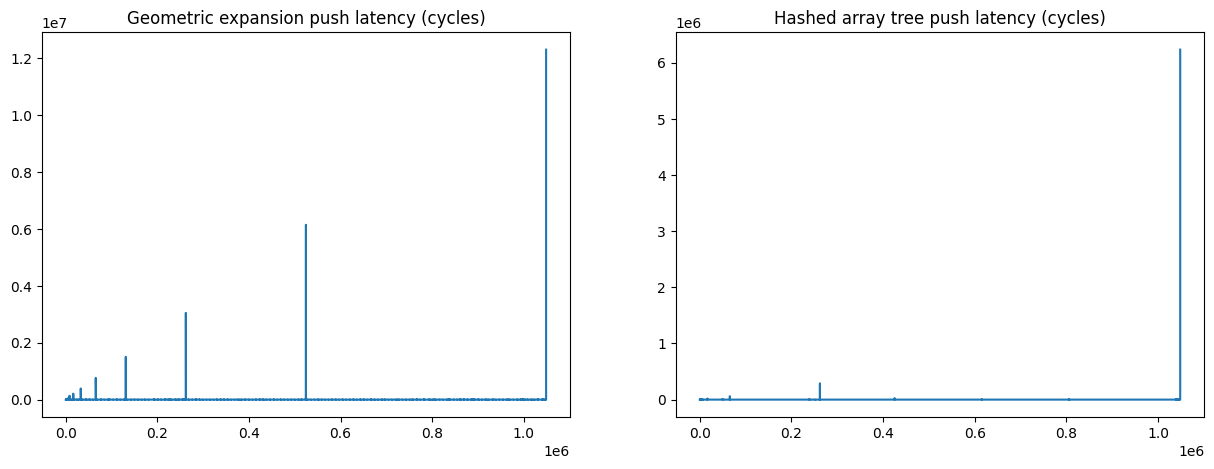
\includegraphics[width=\textwidth]{01-push-latencies.png}
		\caption{Push latencies of different implementations of resizable arrays}
		\label{fig:push-latency}
	\end{figure}
\end{center}

From the axes themselves, it seems like HATs take significantly longer for each of its expansion, especially the later ones since copying elements from one HAT to another is significantly more complicated than copying one array to another in the implementation with geometric expansion (GE). However, the frequency of HATs expanding is significantly lower than with GE as there aren't many latency spikes in the HAT compared to the GE as it clearly has more latency spikes than HATs.

\endgroup

\begingroup

\subsection{Access Latency}

\begin{center}
	\begin{figure}[H]
		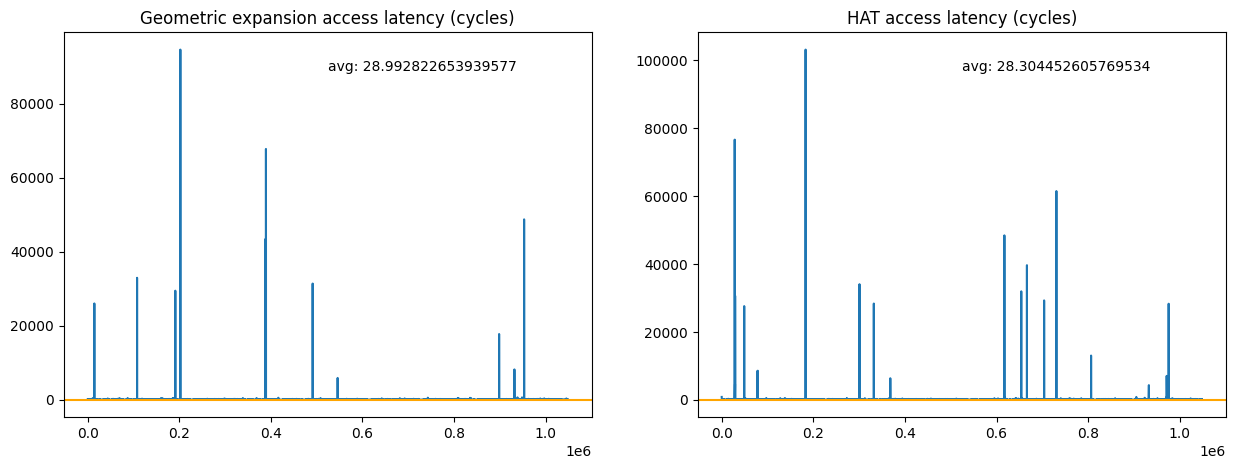
\includegraphics[width=\textwidth]{01-access-latencies.png}
		\caption{Random access latencies of different implementations of resizable arrays}
		\label{fig:get-latency}
	\end{figure}
\end{center}

\endgroup

\begingroup

\subsection{Scan Throughput}

\begin{center}
	\begin{figure}[H]
		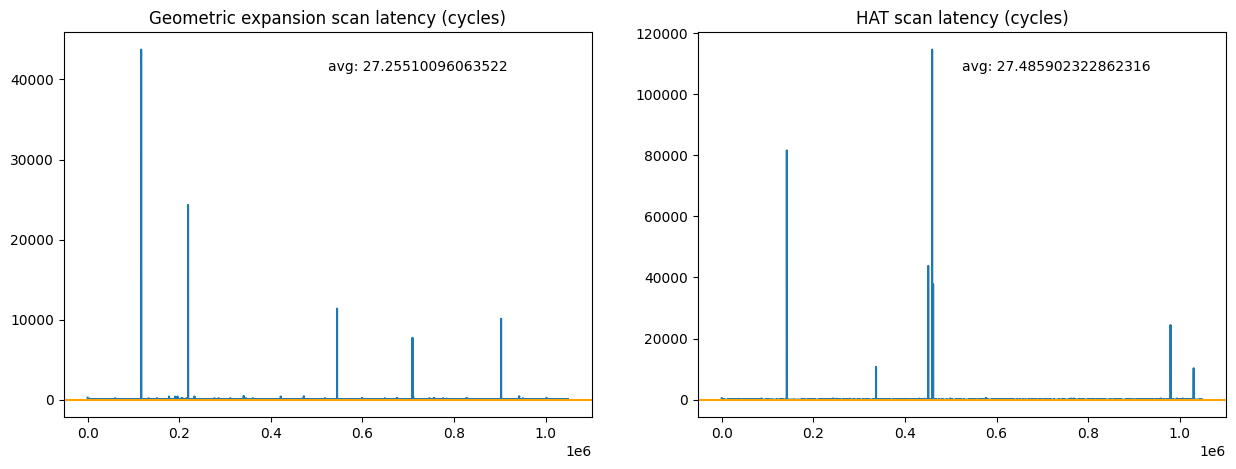
\includegraphics[width=\textwidth]{01-scan-throughput.png}
		\caption{Scan throughput of different implementations of resizable arrays}
		\label{fig:scan-throughput}
	\end{figure}
\end{center}

\endgroup

\begingroup

\subsection{Overall Throughput}

\begin{center}
	\begin{figure}[H]
		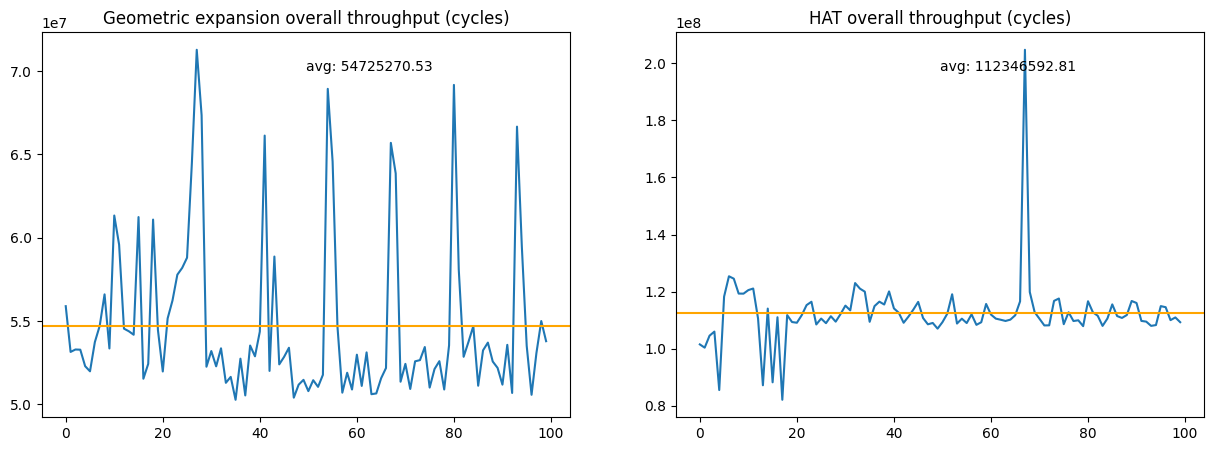
\includegraphics[width=\textwidth]{01-overall-throughput.png}
		\caption{Overall throughput of different implementations of resizable arrays}
		\label{fig:overall-throughput}
	\end{figure}
\end{center}

\endgroup
